\documentclass[slidestop]{beamer}
\usepackage{beamerthemesplit}
\usepackage{graphics}
\usepackage{pstricks}

\title{SIMD}
\author{Rishabh Jain}
\author{Luke Kenneth Casson Leighton}


\begin{document}

\frame{
   \begin{center}
    \huge{Pin Multiplexer}\\
    \vspace{32pt}
    \Large{Auto-generating documentation, code \\
			and resources for a Pinmux}\\
    \vspace{24pt}
    \Large{[proposed for] Chennai 9th RISC-V Workshop}\\
    \vspace{16pt}
    \large{\today}
  \end{center}
}


\frame{\frametitle{Credits and Acknowledgements}

 \begin{itemize}
   \item TODO\vspace{10pt}
  \end{itemize}
}


\frame{\frametitle{Glossary}

 \begin{itemize}
   \item Pin: an I/O pad.  May be driven (input) or may drive (output).
   \item FN: term for a single-wire "function", such as UART\_TX,
	     I2C\_SDA, SDMMC\_D0 etc.  may be an input, output or both
		 (bi-directional: separate wires are always allocated).
   \item TODO\vspace{10pt}
  \end{itemize}
}


\frame{\frametitle{Muxer cases to handle}

 \begin{itemize}
   \item Many FN outputs to Many Pins: no problem\\
	     (weird configuration by end-user, but no damage to ASIC)\vspace{10pt}
   \item One Pin to Many FN inputs: no problem\\
         (weird configuration by end-user, but no damage to ASIC)\vspace{10pt}
   \item Many Pins to One FN input {\bf Priority Mux needed}\\
	     No priority mux: Pin1 = HI, Pin0 = LO, ASIC is damaged\vspace{10pt}
   \item Some FNs (I2C\_SDA, SD\_D0..3) are I/O Buses\\
	     Bi-directional control of the Pin must be handed to the
	     FN\vspace{10pt}
   \item TODO\vspace{10pt}
  \end{itemize}
}


\frame{\frametitle{Standard GPIO 4-way in/out Mux and I/O pad}
 \begin{center}
  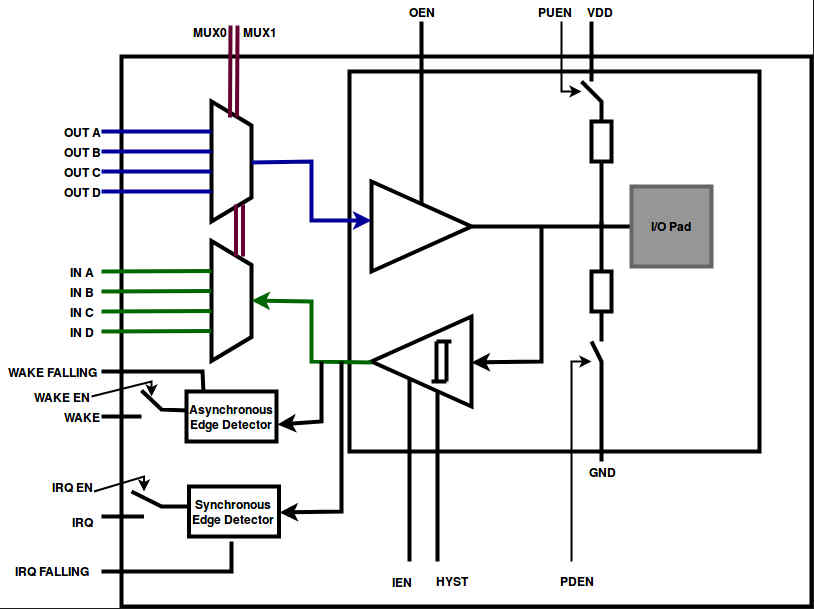
\includegraphics[height=2.5in]{../shakti/m_class/mygpiomux.jpg}\\
  {\bf 4-in, 4-out, pullup/down, hysteresis, edge-detection (EINT)}
 \end{center}
}


\frame{\frametitle{Register-to-pad "control" settings}
 \begin{center}
  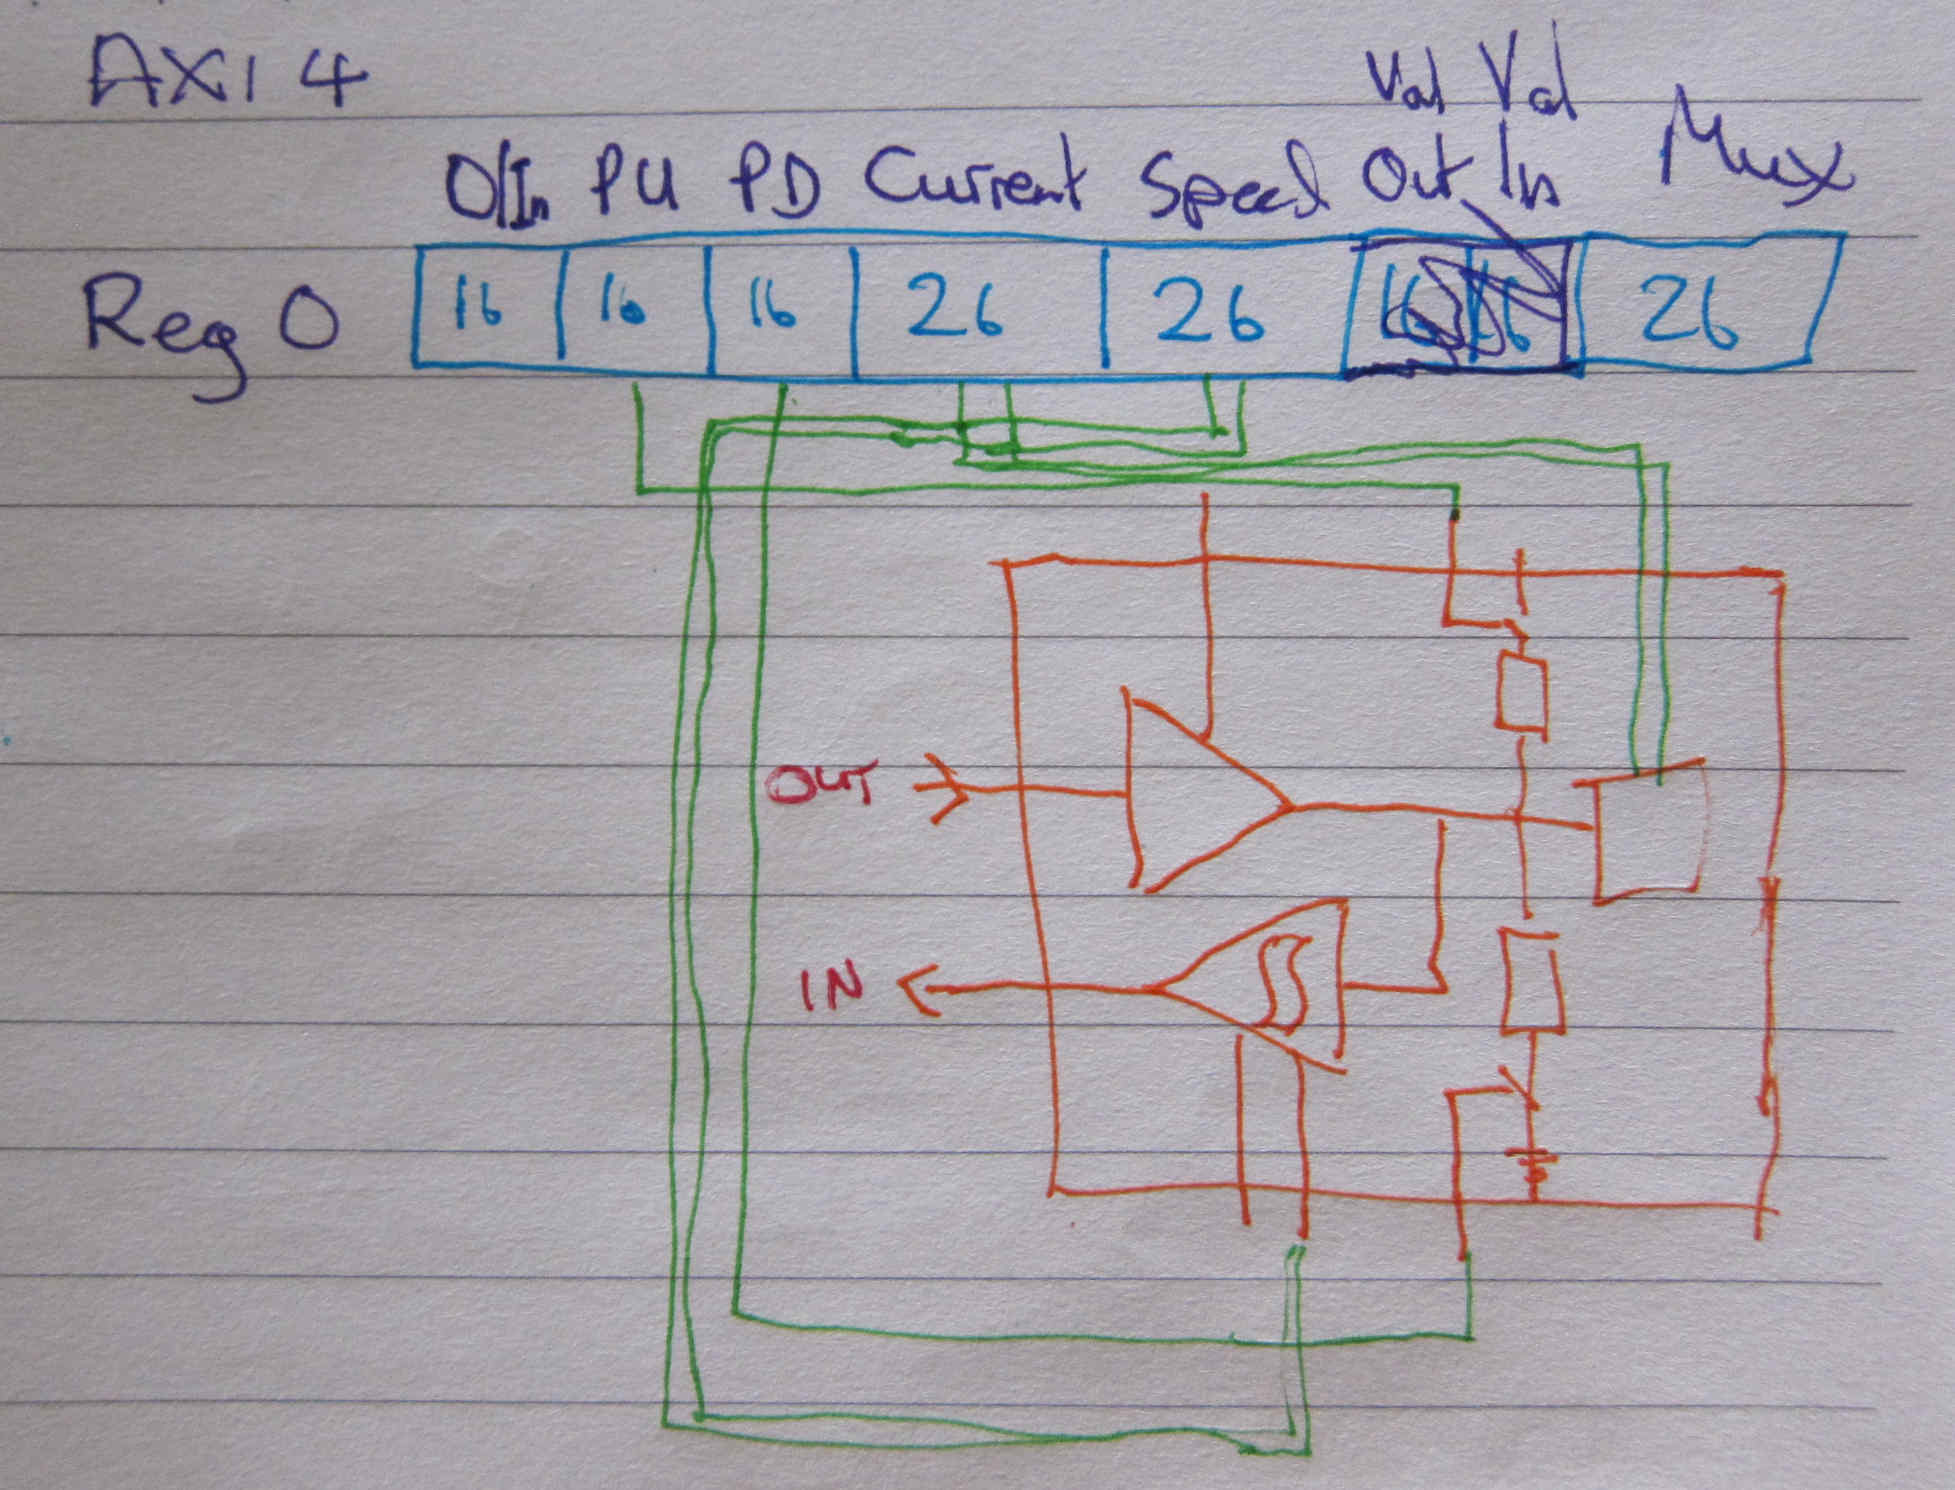
\includegraphics[height=2.5in]{reg_gpio_cap_ctrl.jpg}\\
  {\bf pullup/down, hysteresis, current, edge-detection}
 \end{center}
}


\frame{\frametitle{In/Out muxing, direction control}
 \begin{center}
  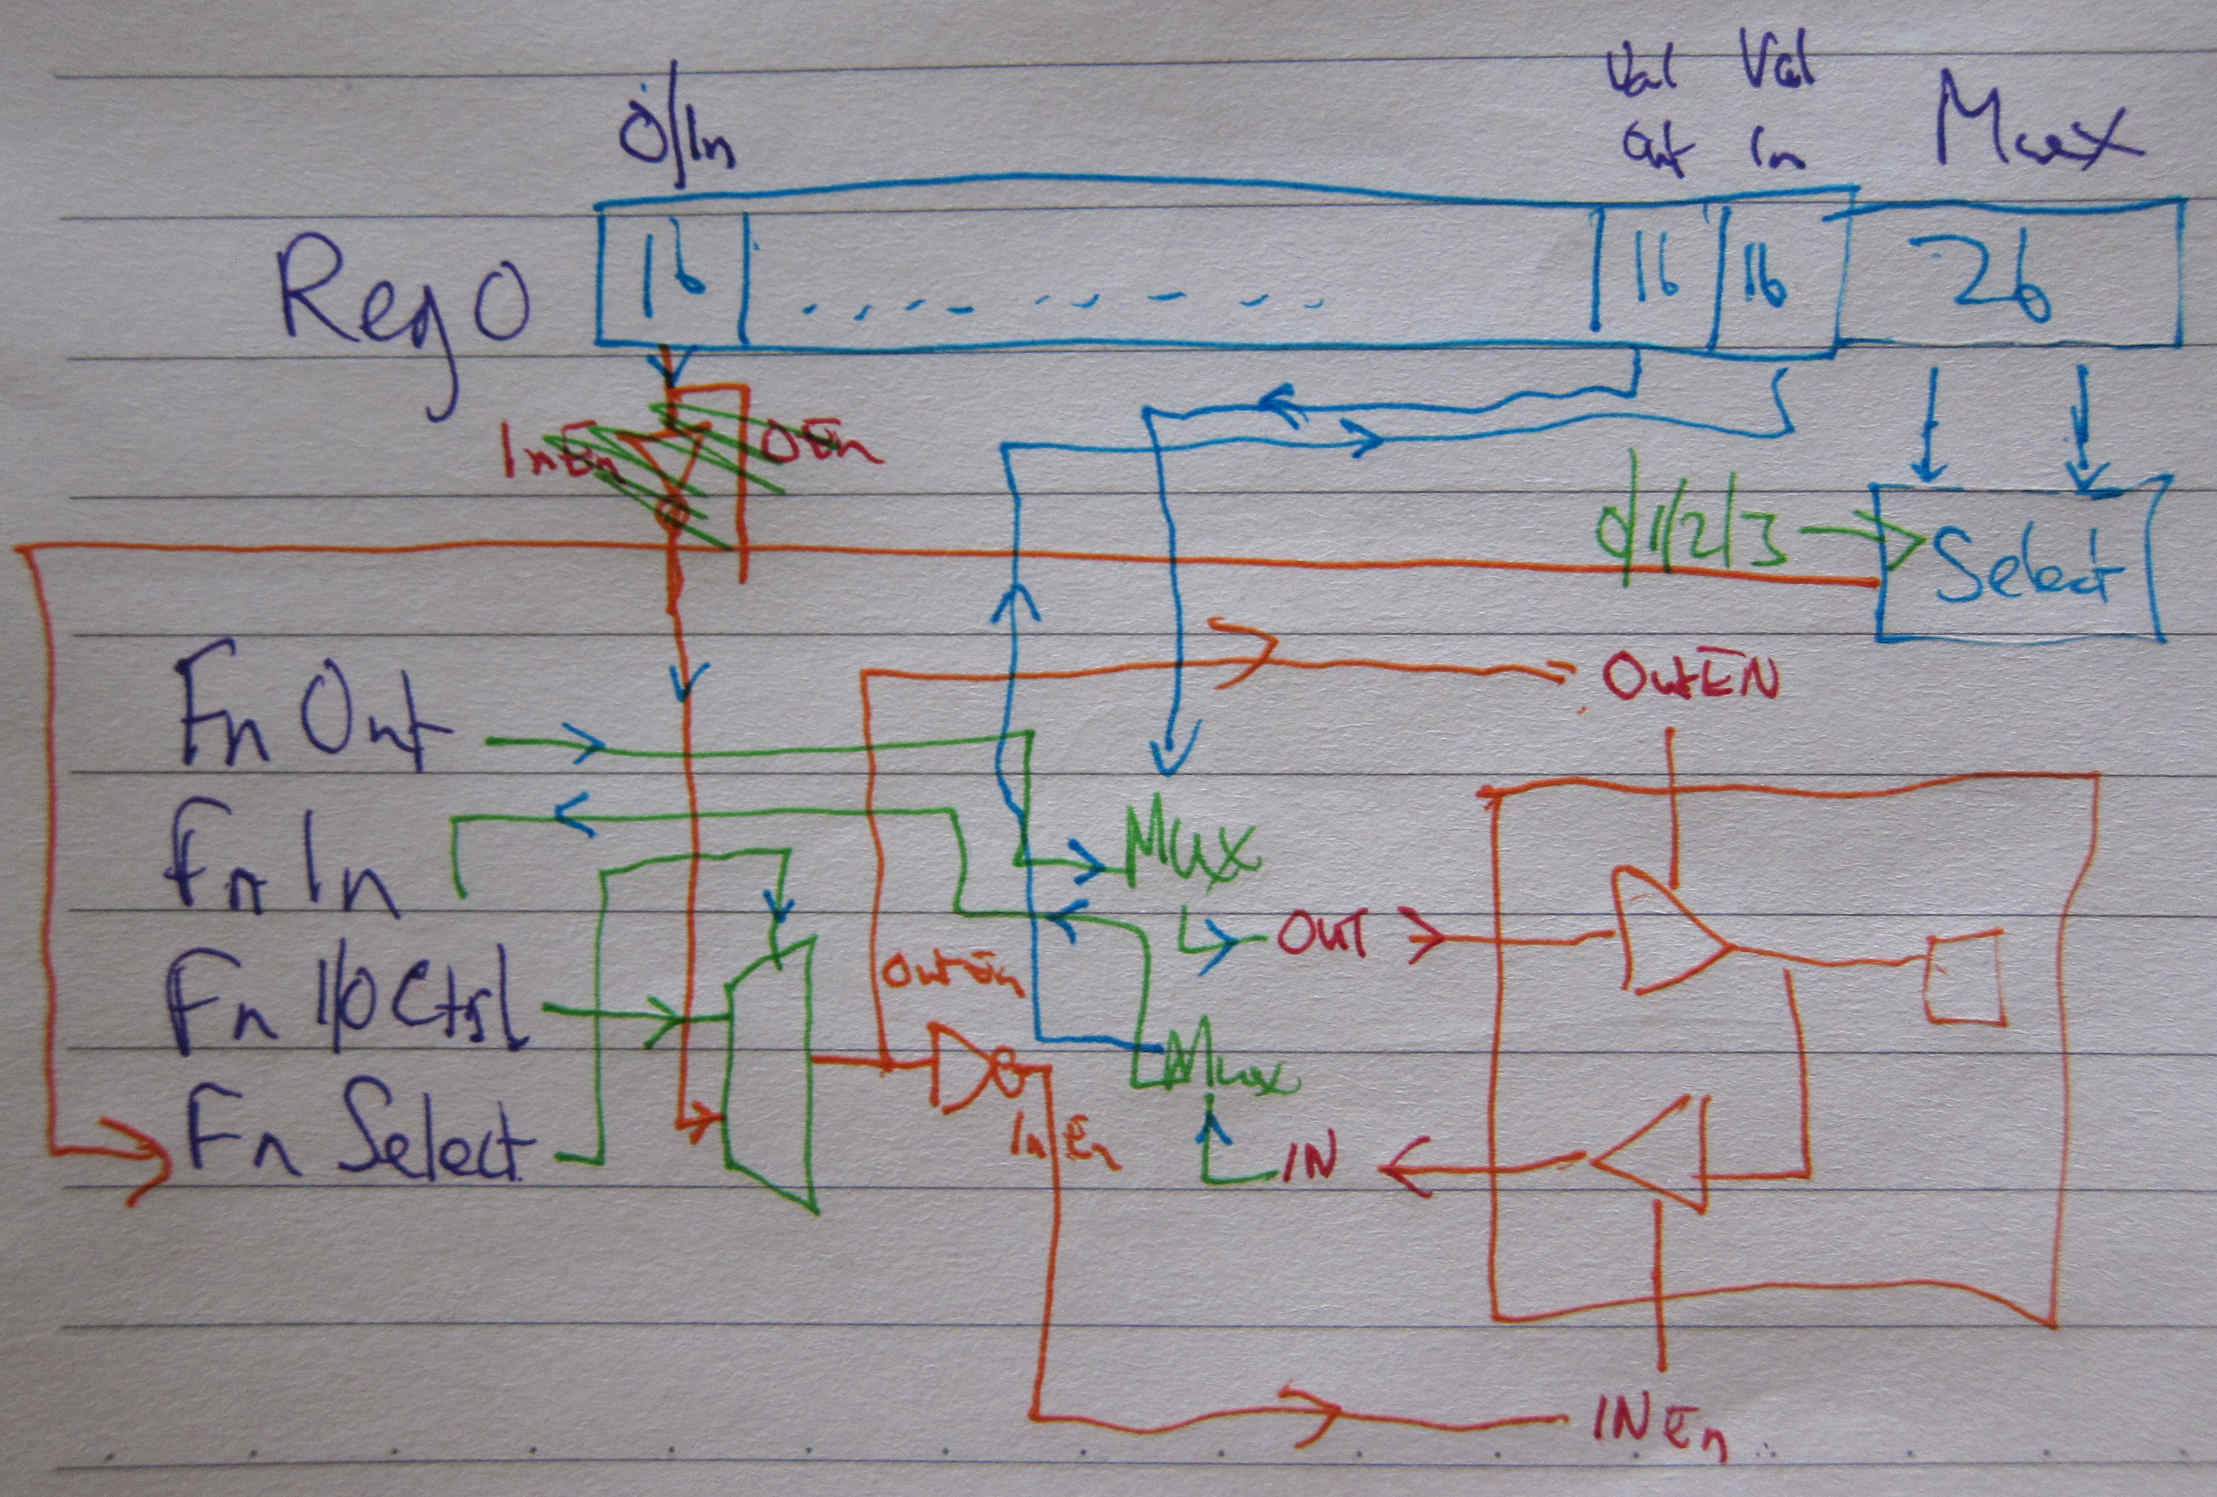
\includegraphics[height=2.5in]{reg_gpio_fn_ctrl.jpg}\\
  {\bf Note: function can control I/O direction}
 \end{center}
}


\frame{\frametitle{Simplified I/O pad Block Diagram}
 \begin{center}
  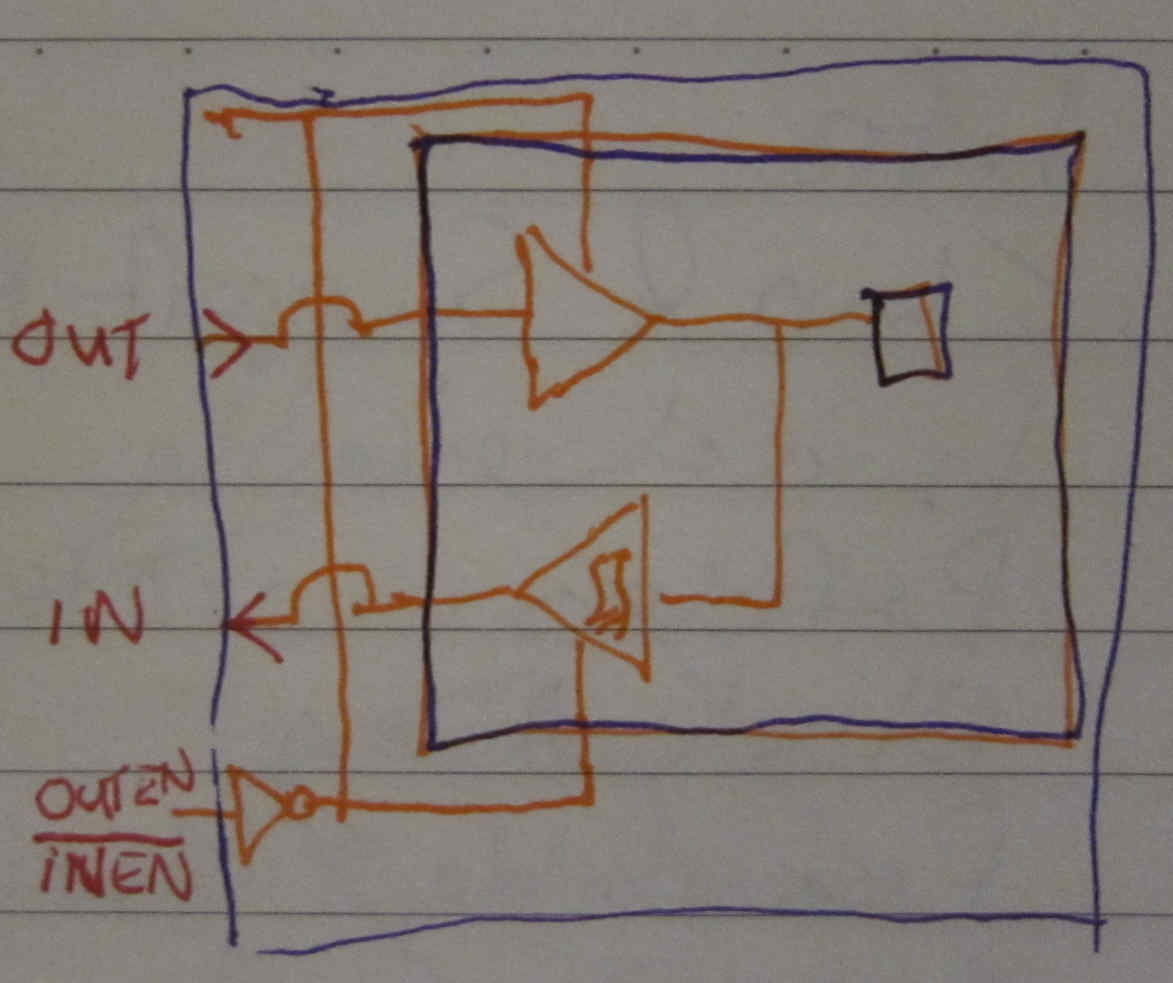
\includegraphics[height=2.5in]{reg_gpio_pinblock.jpg}\\
  {\bf 3 wires: IN, OUT, OUTEN (also = !INEN) }
 \end{center}
}


\frame{\frametitle{Output (and OUTEN) Wiring. 2 pins, 2 GPIO, 2 Fns}
 \begin{center}
  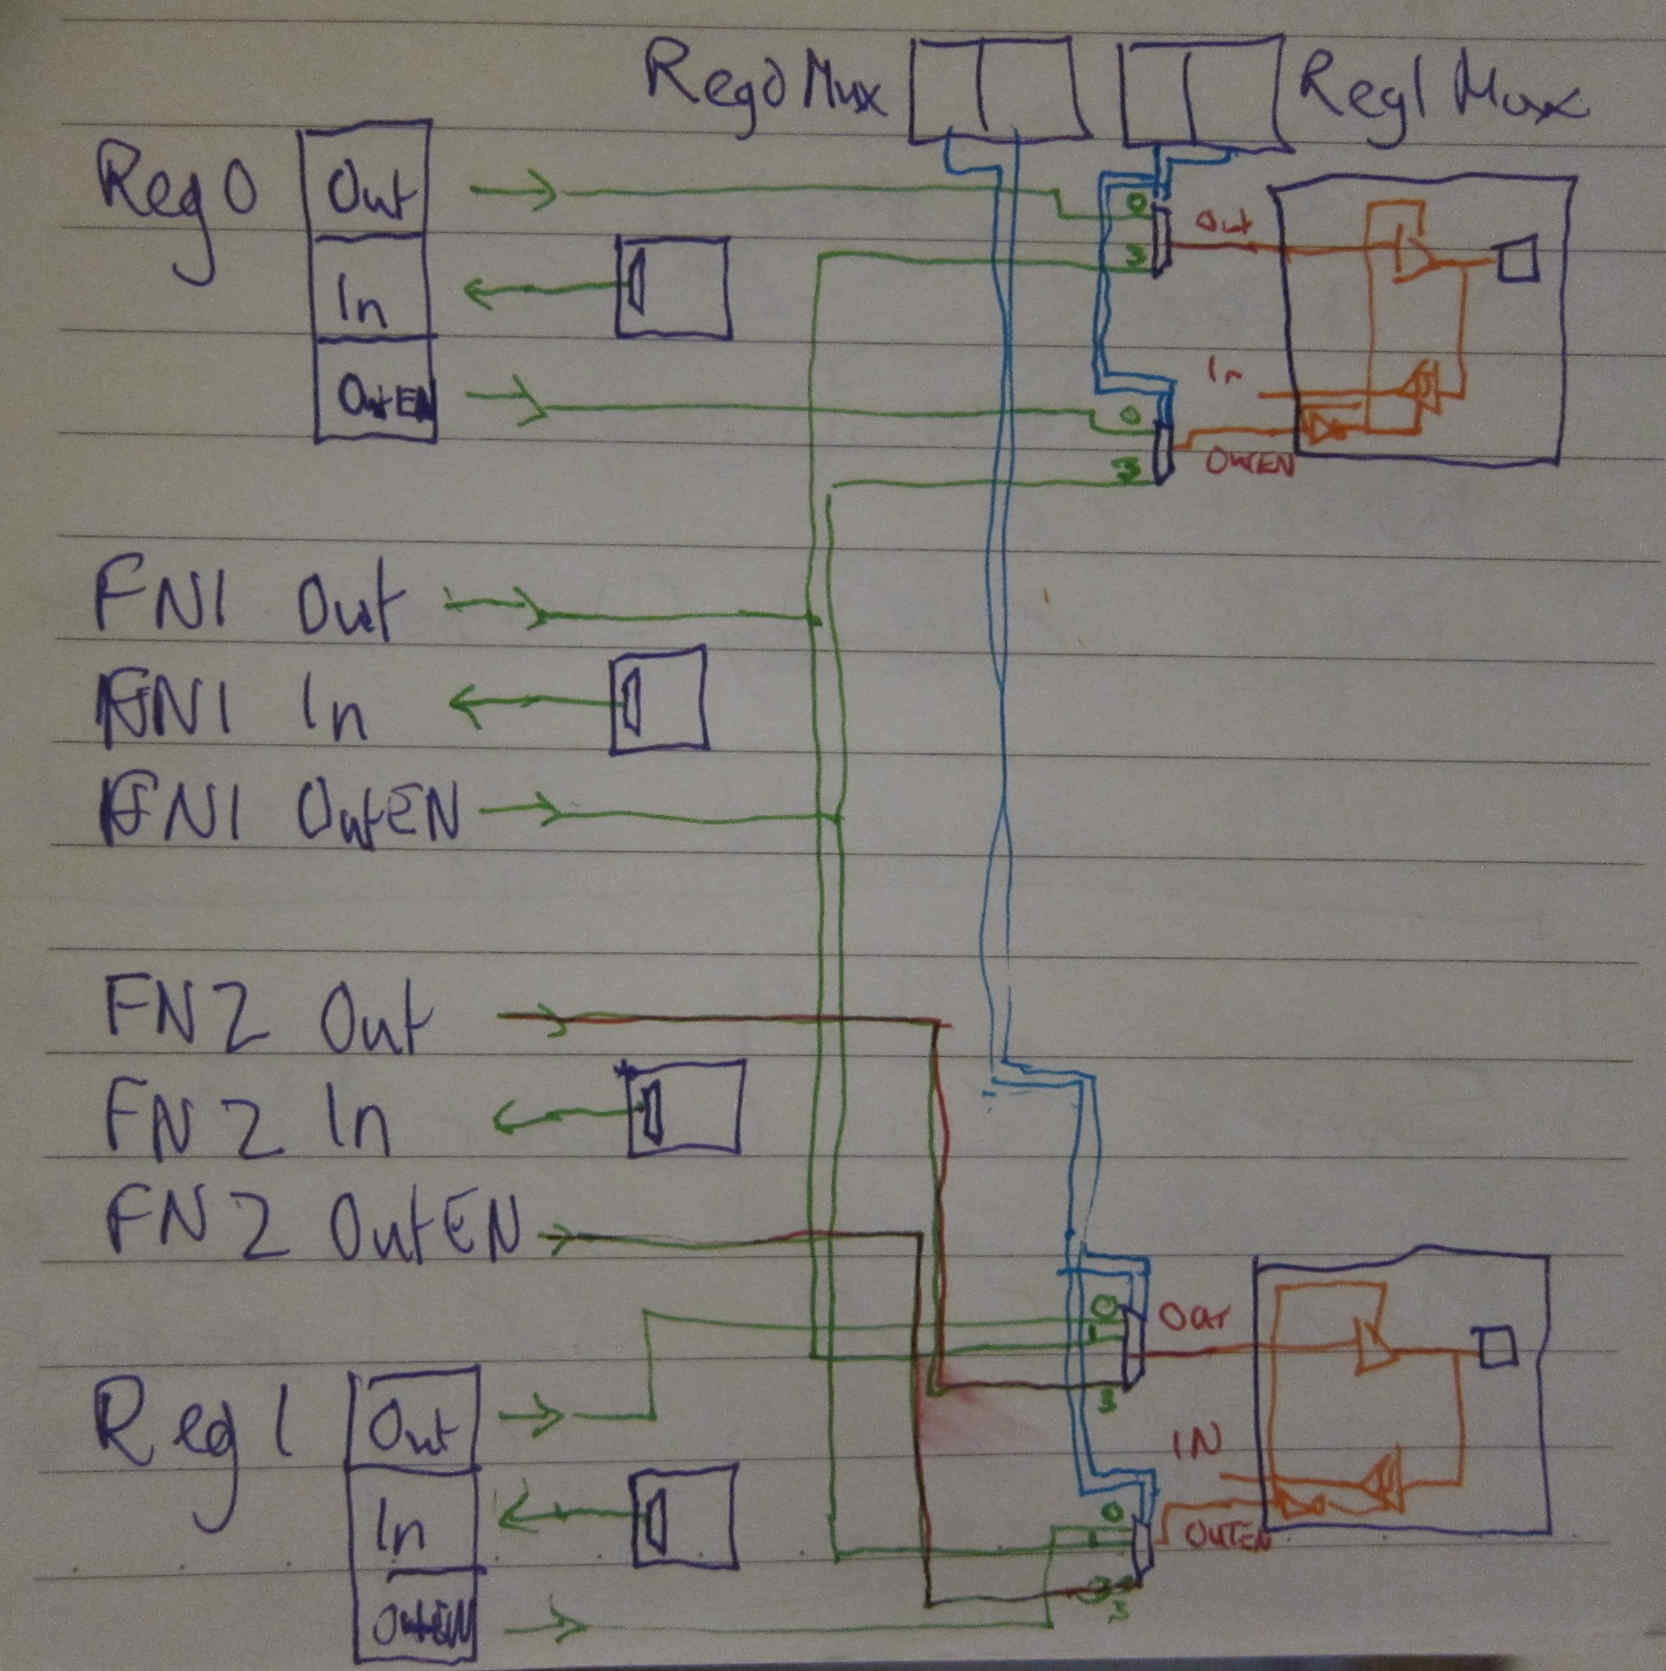
\includegraphics[height=2.5in]{reg_gpio_out_wiring.jpg}\\
  {\bf Reg0 for Pin0, Reg1 for Pin1, Output and OUTEN same mux }
 \end{center}
}


\frame{\frametitle{Input Selection and Priority Muxing}
 \begin{center}
  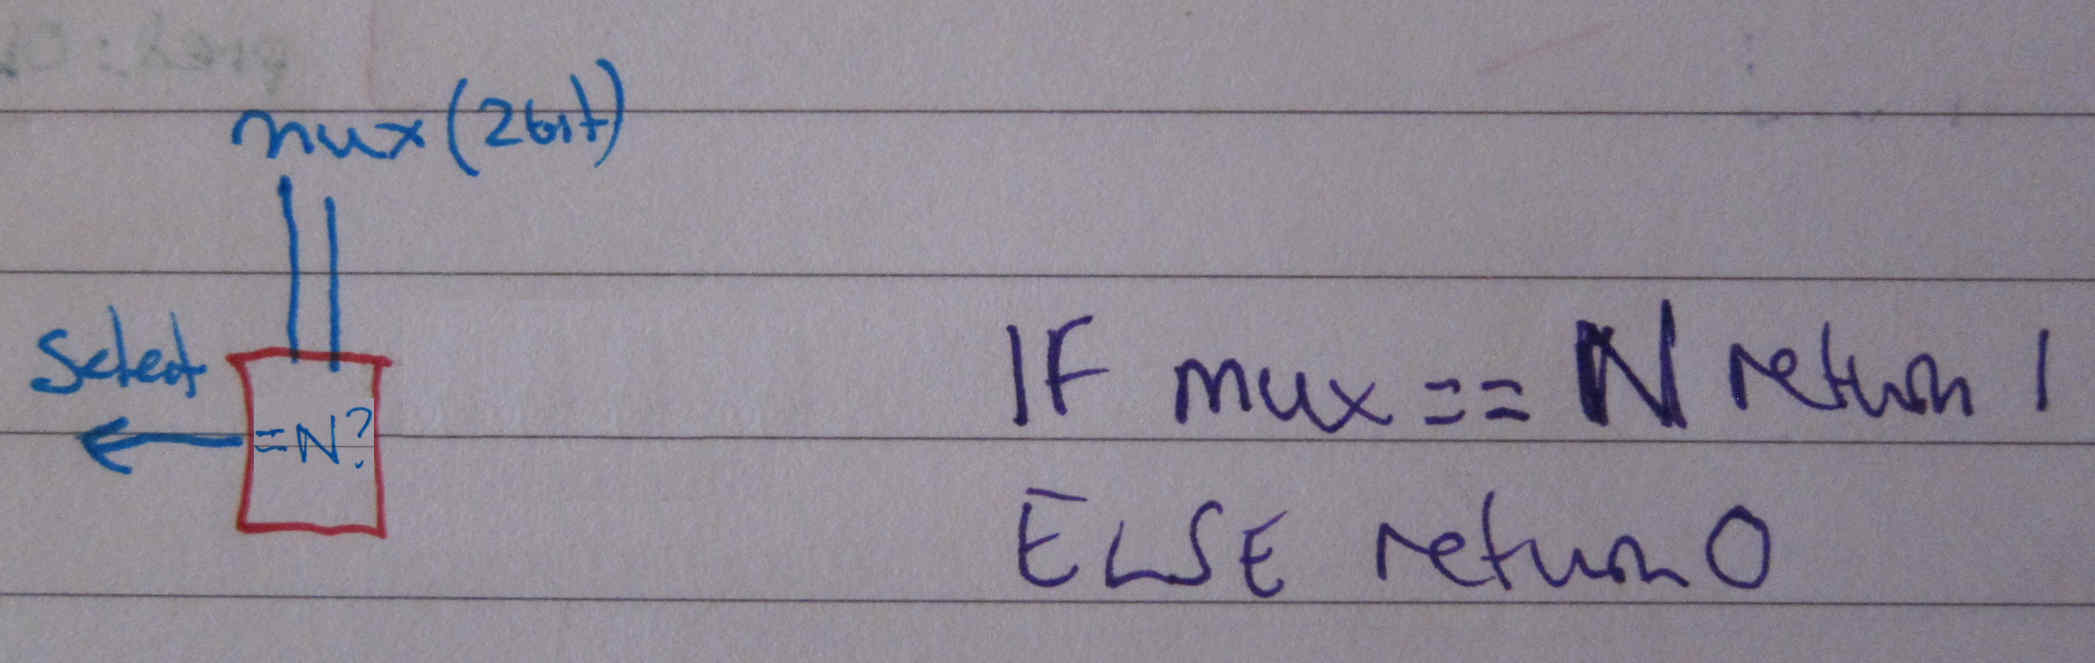
\includegraphics[height=0.75in]{reg_gpio_comparator.jpg}\\
  {\bf Muxer enables input selection}\\
  \vspace{10pt}
  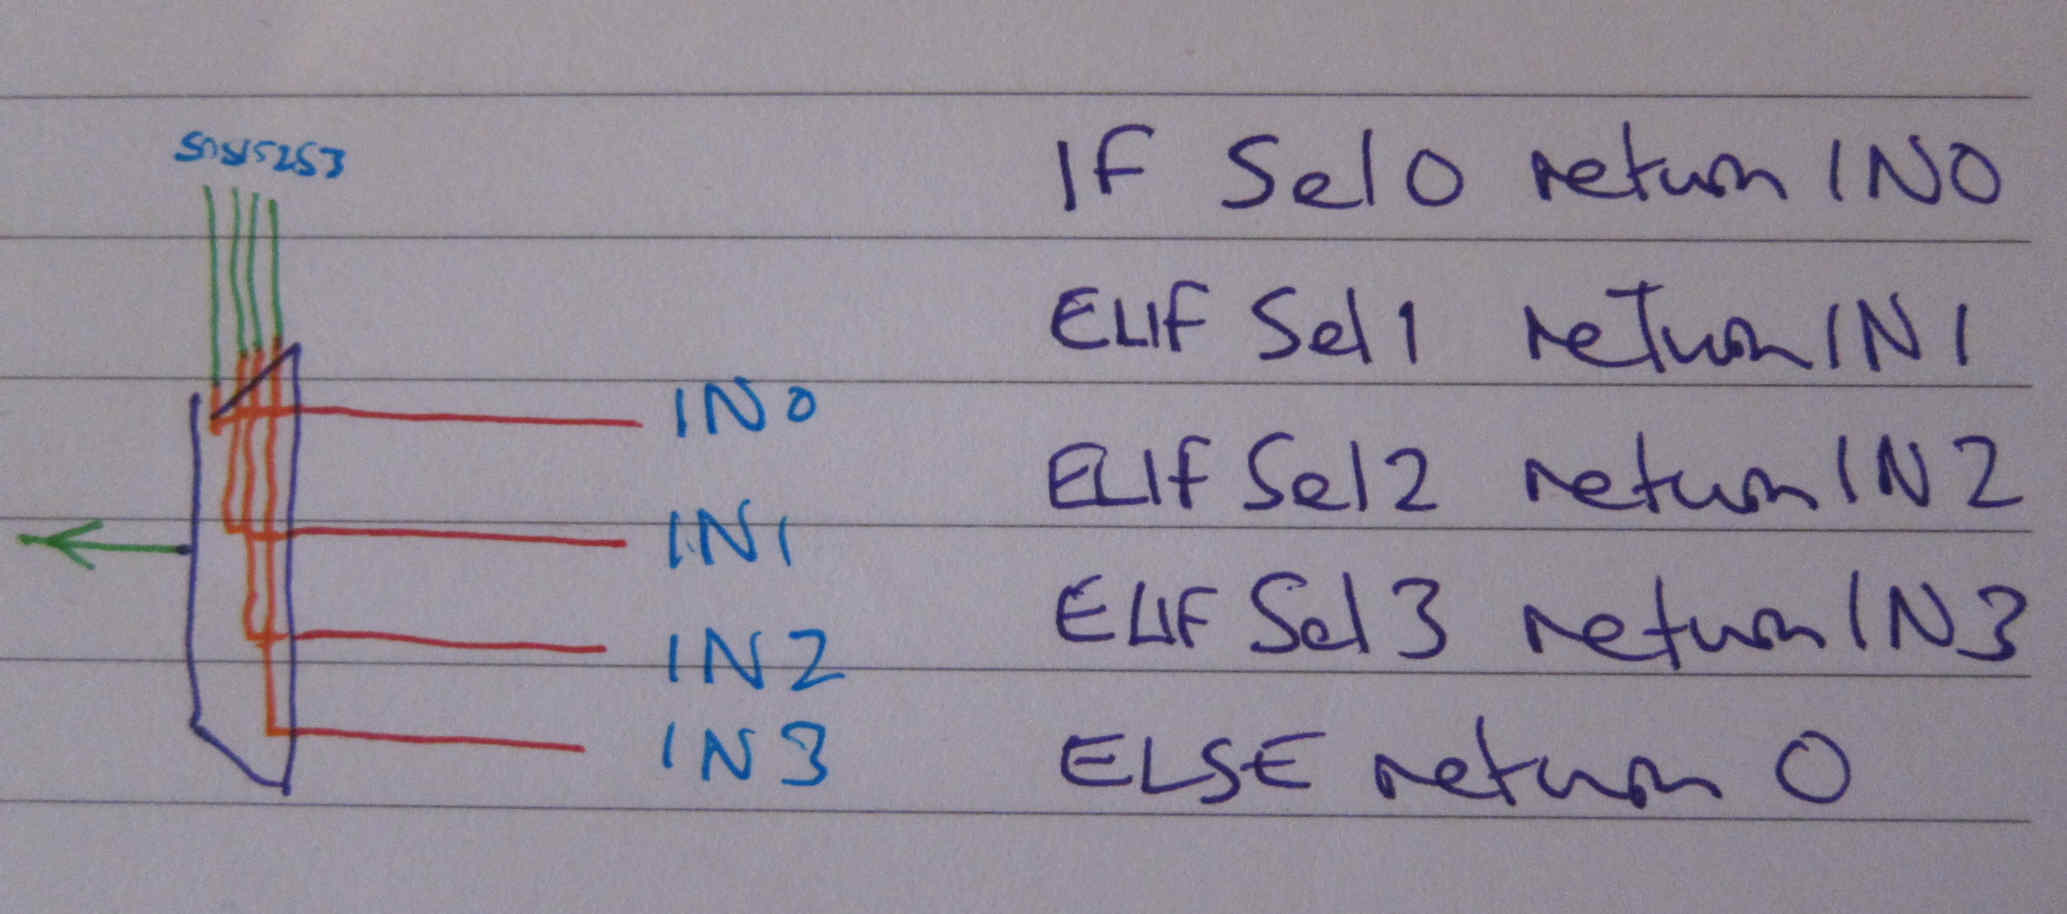
\includegraphics[height=1.25in]{reg_gpio_in_prioritymux.jpg}\\
  {\bf However multiple inputs must be prioritised }
 \end{center}
}


\frame{\frametitle{Input Mux Wiring}
 \begin{center}
  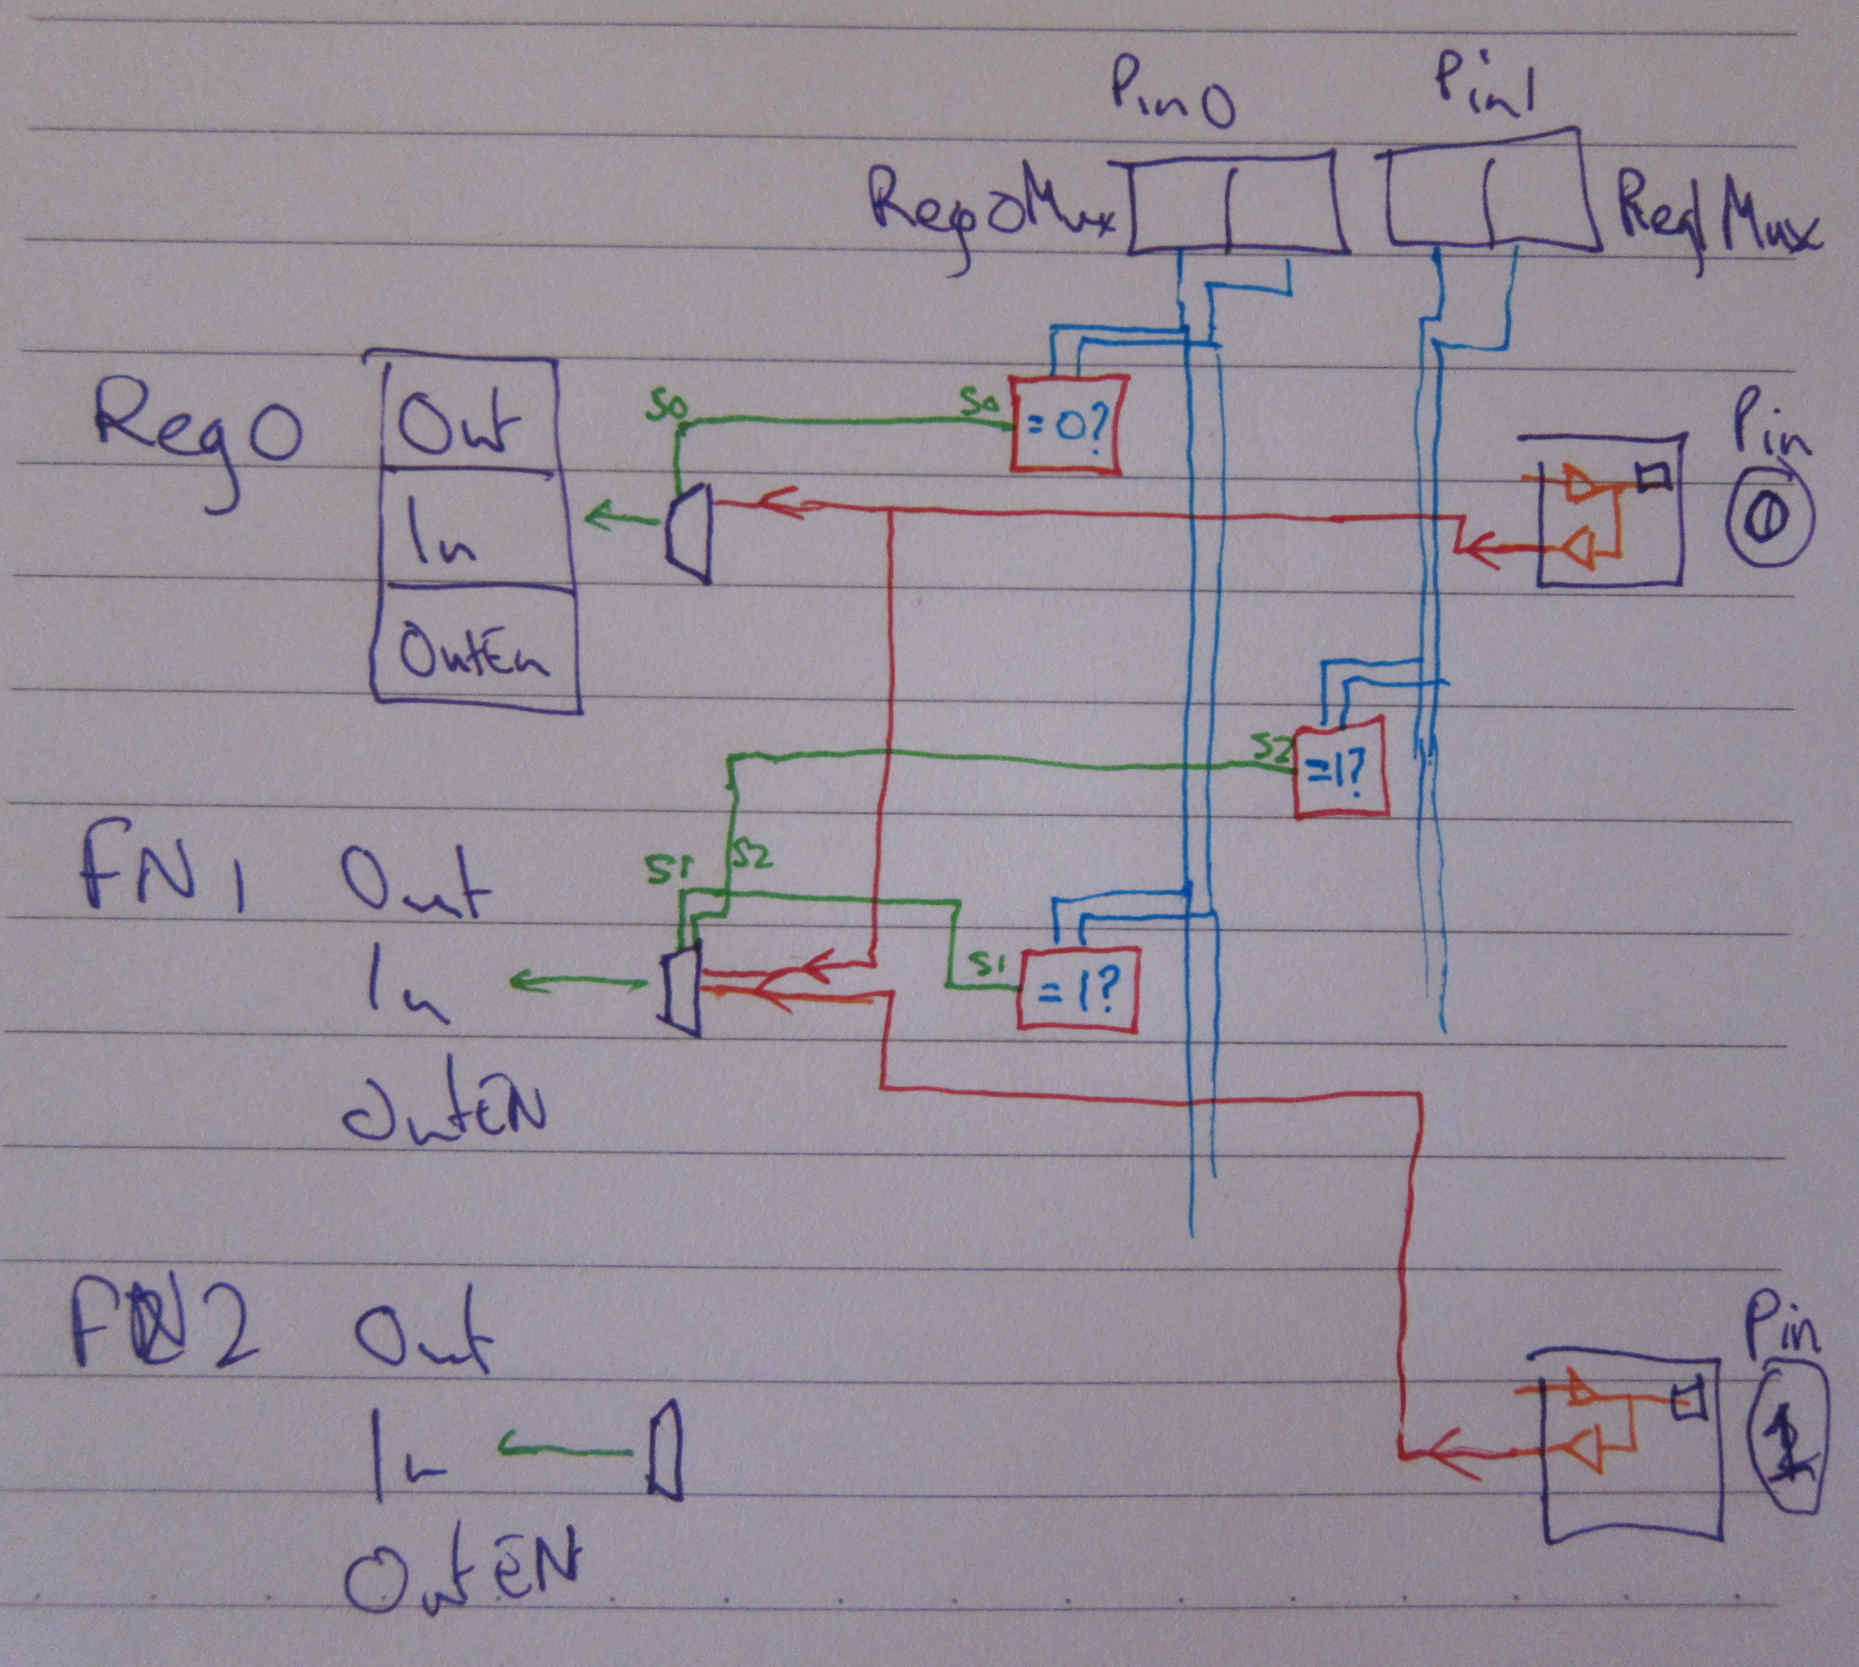
\includegraphics[height=2.5in]{reg_gpio_in_wiring.jpg}\\
  {\bf Pin Mux selection vals NOT same as FN selection vals}
 \end{center}
}


\frame{\frametitle{Summary}

 \begin{itemize}
   \item TODO
  \end{itemize}
}


\frame{
  \begin{center}
    {\Huge The end\vspace{20pt}\\
		   Thank you\vspace{20pt}\\
		   Questions?\vspace{20pt}
	}
  \end{center}
  
  \begin{itemize}
	\item http://libre-riscv.org/shakti/m\_class/pinmux/
  \end{itemize}
}


\end{document}
